To attempt at reconstructing the truth from a noisy observation, it is essential to understand the underlying noise statistics. Classical and quantum optics provide a comprehensive theoretical foundation to explain photon statistics. For instance, it is well understood that photons from a coherent light source follow a Poisson distribution, often referred to as shot-noise. Whereas, for chaotic (bunched) light, the variance exceeds that compared to their mean, dubbed super-Poissonian. And finally for a squeezed light source, the distribution is sub-Poissonian \cite[Chapter~5]{foxQuantumOpticsIntroduction2006}.

In this chapter, we start with defining the Poisson model for counting photo-electron event data. We examine our data to identify where this model is appropriate and where its limitations become evident. To this end, we introduce some statistical apparatus necessary to estimate parameters and define goodness of model. Further, we explore why the \gls{FEL} light source (see section \ref{section:light-sources}), exhibits over-dispersed statistics, a characteristic necessitating moving beyond the Poisson model. Accounting for this, we transition to using the Negative Binomial distribution as a more suitable model for the count data. Lastly, we acknowledge that theoretically these models primarily address photon statistics and a more sophisticated treatment building on light-matter interaction might be necessary to connect photon statistics with the statistics of the emitted electrons.

\section{Poisson distribution as a model for counting statistics}

To model counting of independently occurring events, the Poisson distribution is often used. The discrete probability distribution expresses the probability of a given number of events occurring in a fixed interval of time, space or other domains\cite{fellerIntroductionProbabilityTheory1968}:
\begin{note}
    {Poisson distribution}
    The \gls{PMF} for Poisson distribution Poi\((\lambda)\) with \(\lambda > 0\) is defined as
    \begin{equation}
        P(n;\lambda) = \frac{\lambda^n e^{-\lambda}}{n!}, \quad n \in \mathbb{N}_0
    \end{equation}
    \begin{enumerate}
        \item $\lambda = E(X) = Var(X)$ 
        \item Additivity: If $X_1 \sim \text{Poi}(\lambda_1)$ and $X_2 \sim \text{Poi}(\lambda_2)$ are independent Poisson random variables, then the sum $X_1 + X_2$ also follows a Poisson distribution with parameter $\lambda_1 + \lambda_2$
        \begin{equation}
            X_1 + X_2 \sim \text{Poi}(\lambda_1 + \lambda_2).
        \end{equation}
        
        This property is useful when considering counts from multiple independent sources.
    \end{enumerate}
\end{note}


\section{Correlated events in detector}



There's a lot of parameters that need to be tested to determine what sort of counting statistics the dataset has.

Controls for the test:
lets see
\begin{itemize}
    \item Total time being looked at (like 1000 s or 20 hours)
    \begin{itemize}
        \item distribution might change due to overtime FEL intensity changes
    \end{itemize}
    \item Time bins being used (like 2 s vs 20 s and so on).
    \begin{itemize}
        \item Seems like distribution changes based on that too
    \end{itemize}
    \item Looking at individual pixels on X and Y
    \item Looking at Energy axis as it behaves weirder
    \item Looking at a larger region in X and Y 
    \begin{itemize}
        \item should follow same statisitics as single pixels
    \end{itemize}
    \item Check after removing correlated electrons within each pulse
    \begin{itemize}
        \item It is possible that electrons are correlated between different pulses because the time delay is long enough. But seems highly unlikely!
    \end{itemize}
    \begin{itemize}
        \item 
    \end{itemize}
\end{itemize}


\subsection{Before filtering}

\begin{figure}
    \centering
    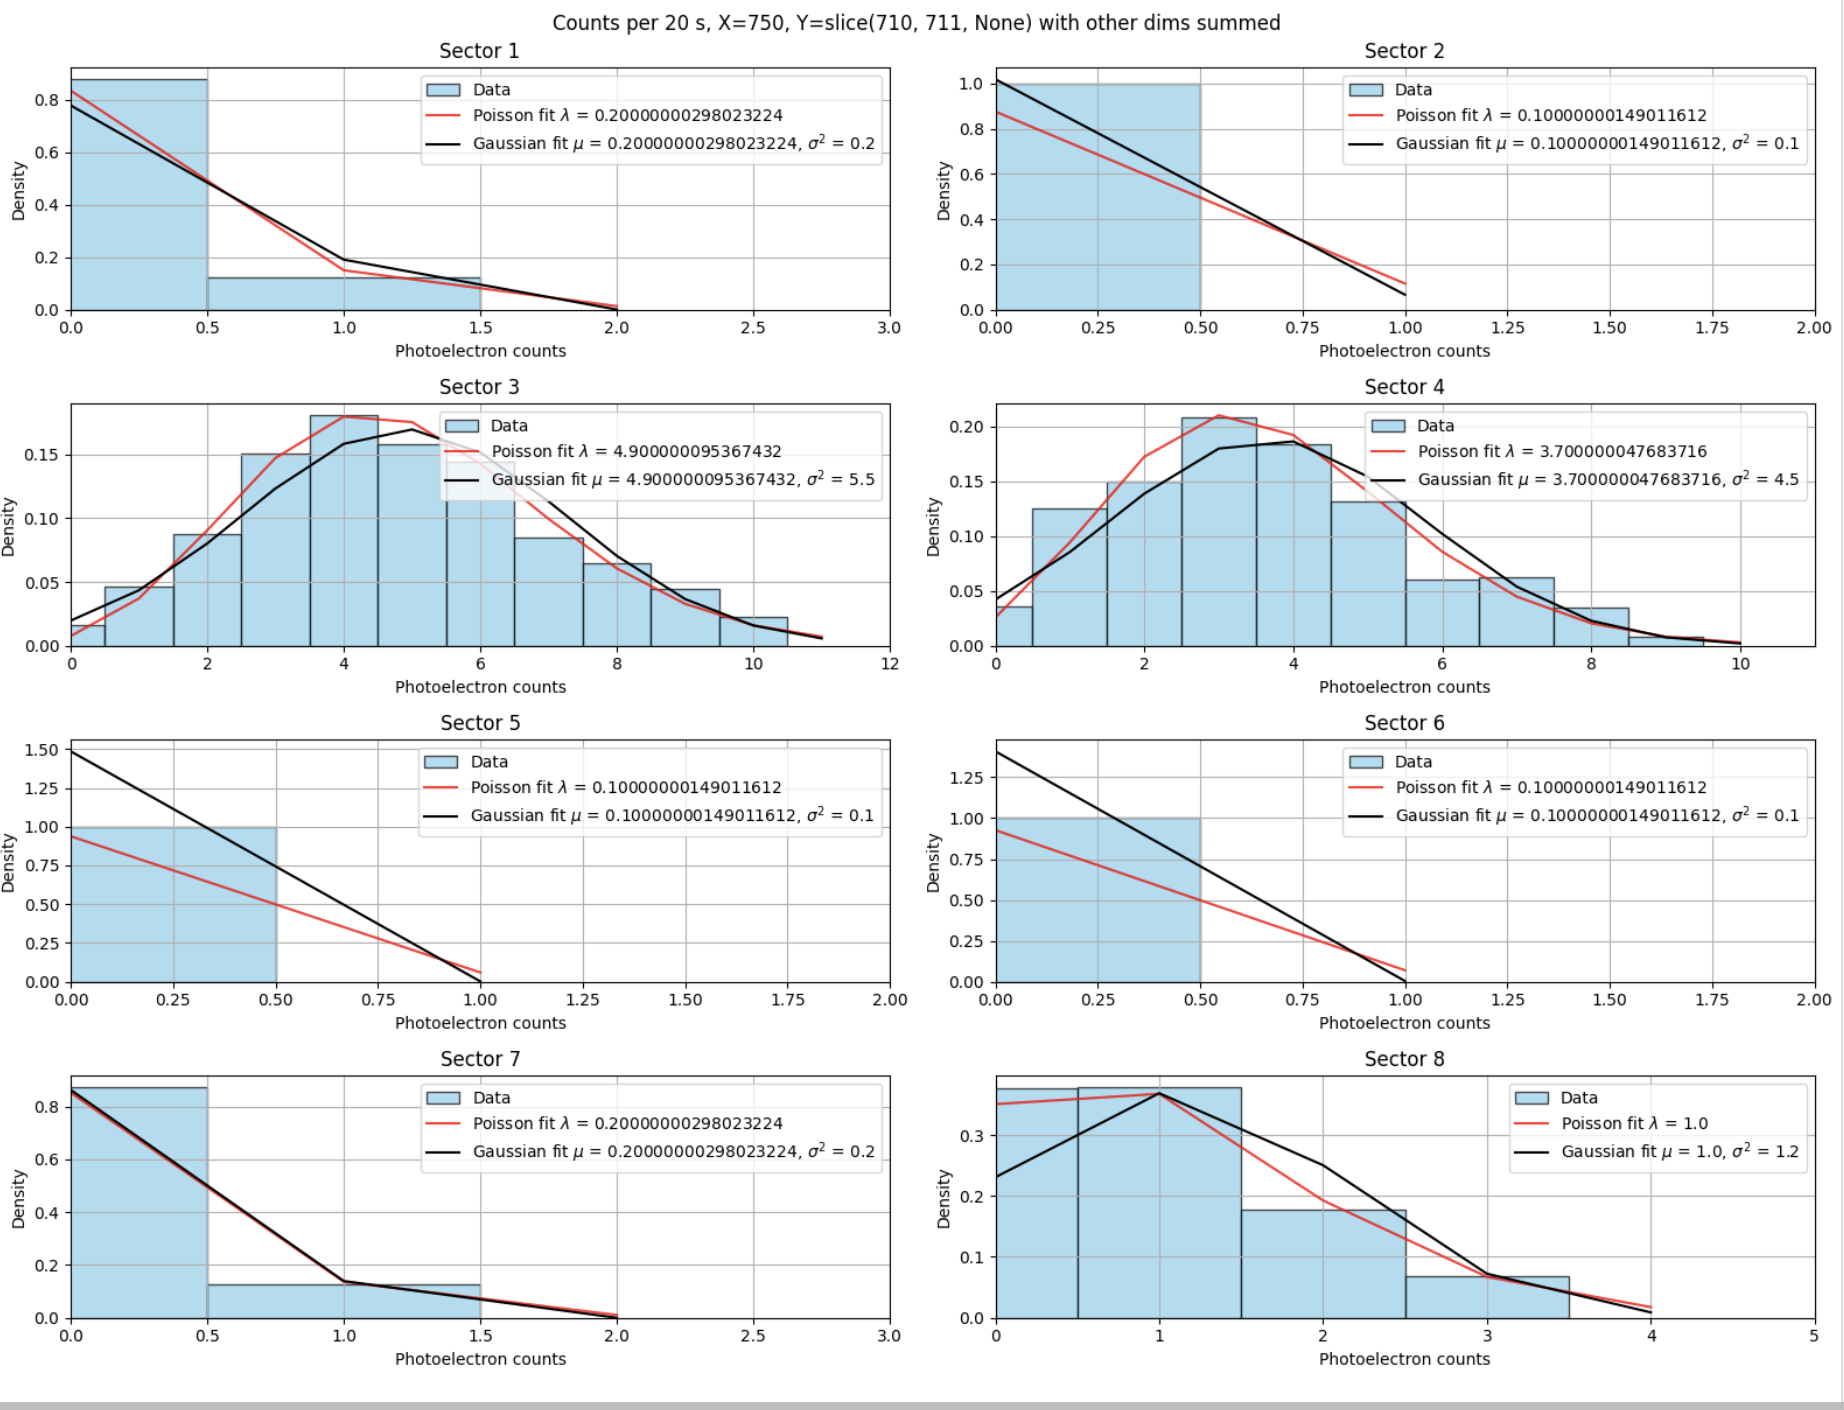
\includegraphics[width=1\linewidth]{images/image.png}
    \caption{Enter Caption}
    \label{Image at one 2D pixel but summed over energy}
\end{figure}

\begin{figure}
    \centering
    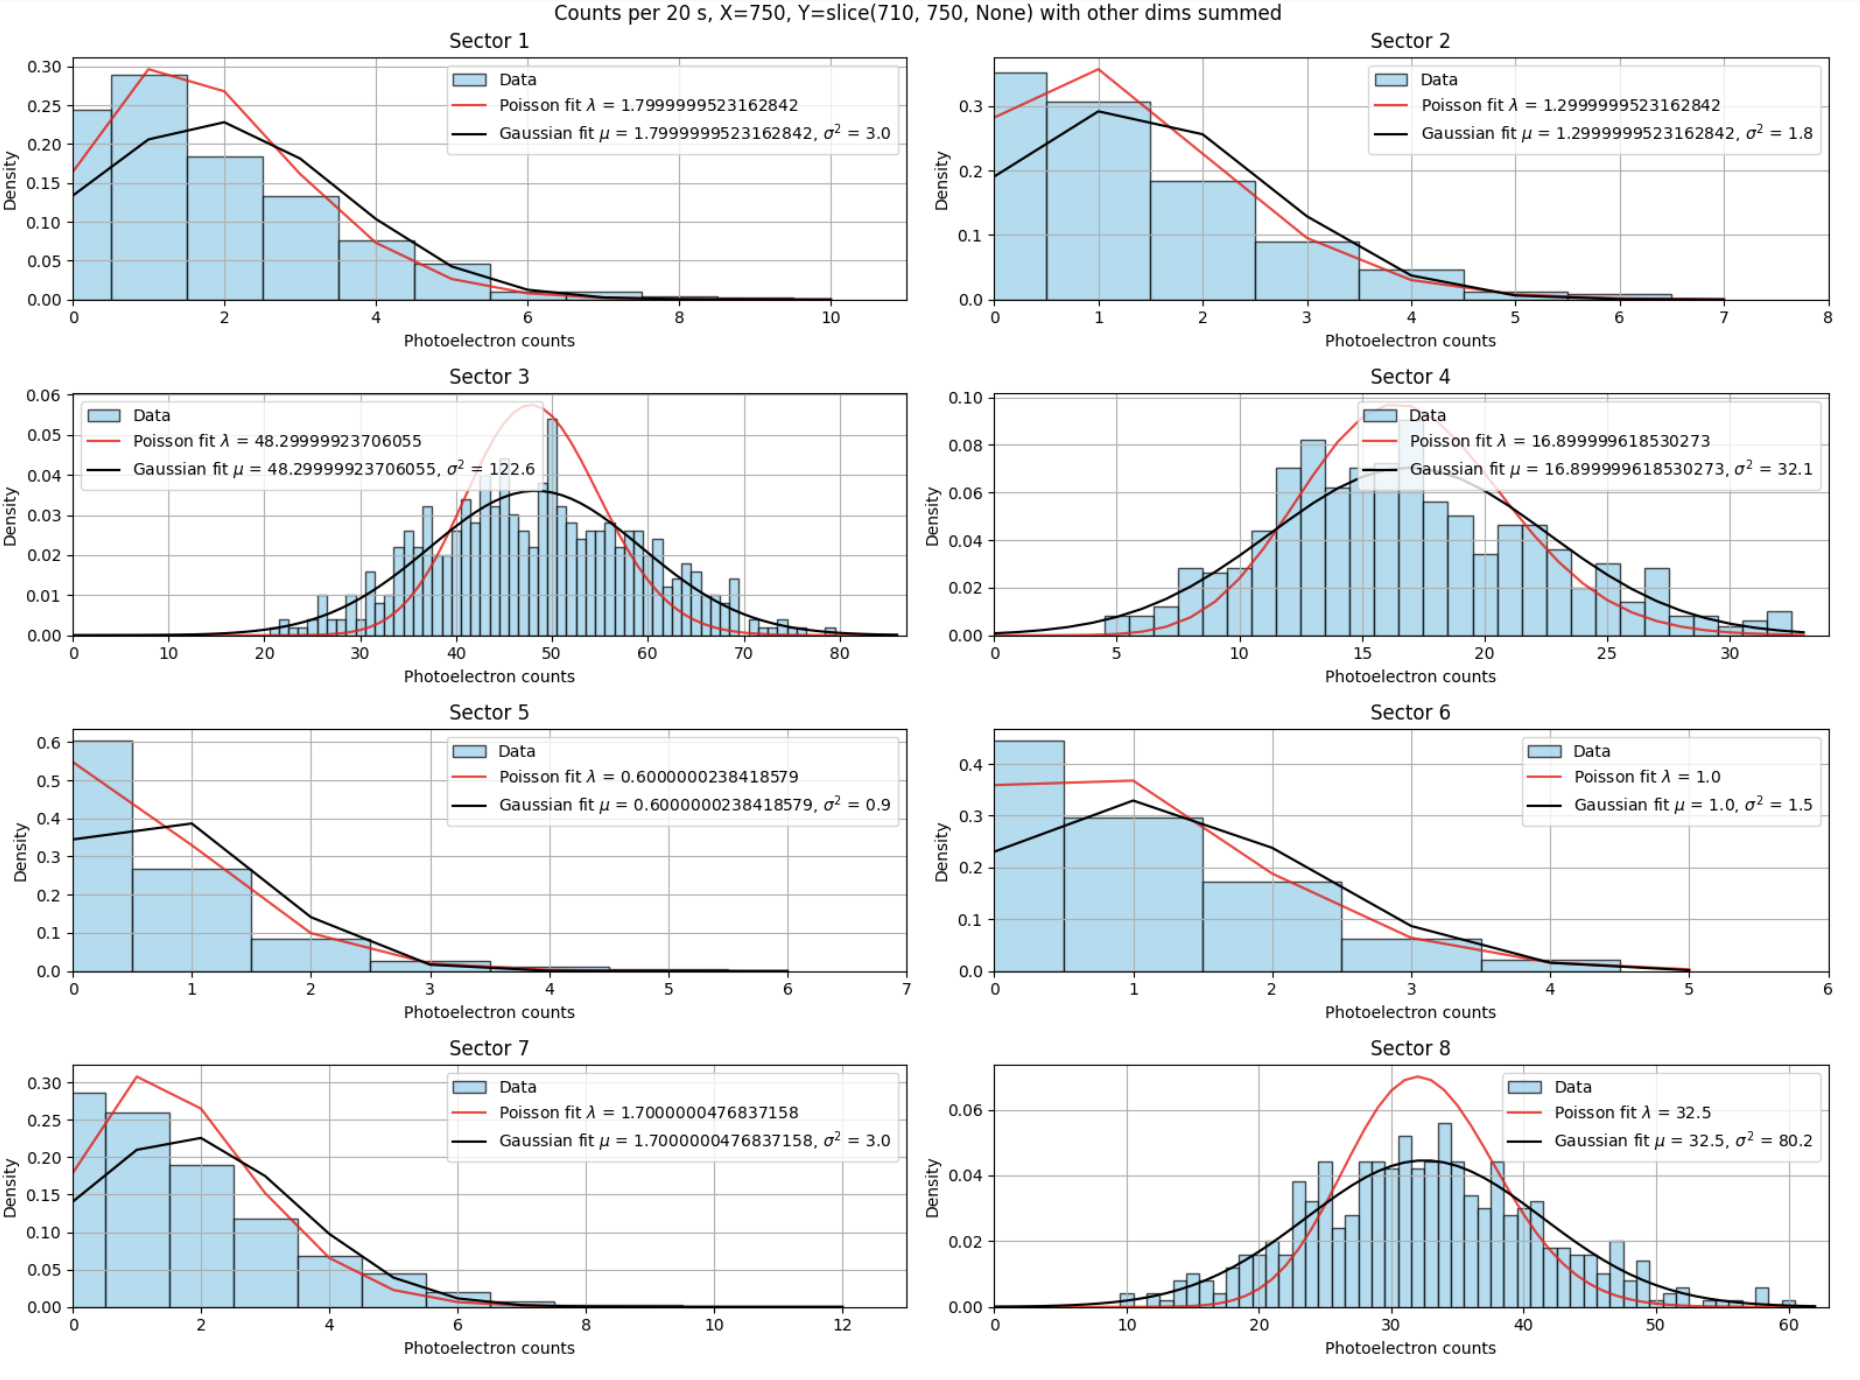
\includegraphics[width=1\linewidth]{images/summed.png}
    \caption{Image over 40 pixels and summed over energy}
    % \label{fig:enter-label}
\end{figure}

\subsection{After filtering}

\begin{figure}
    \centering
    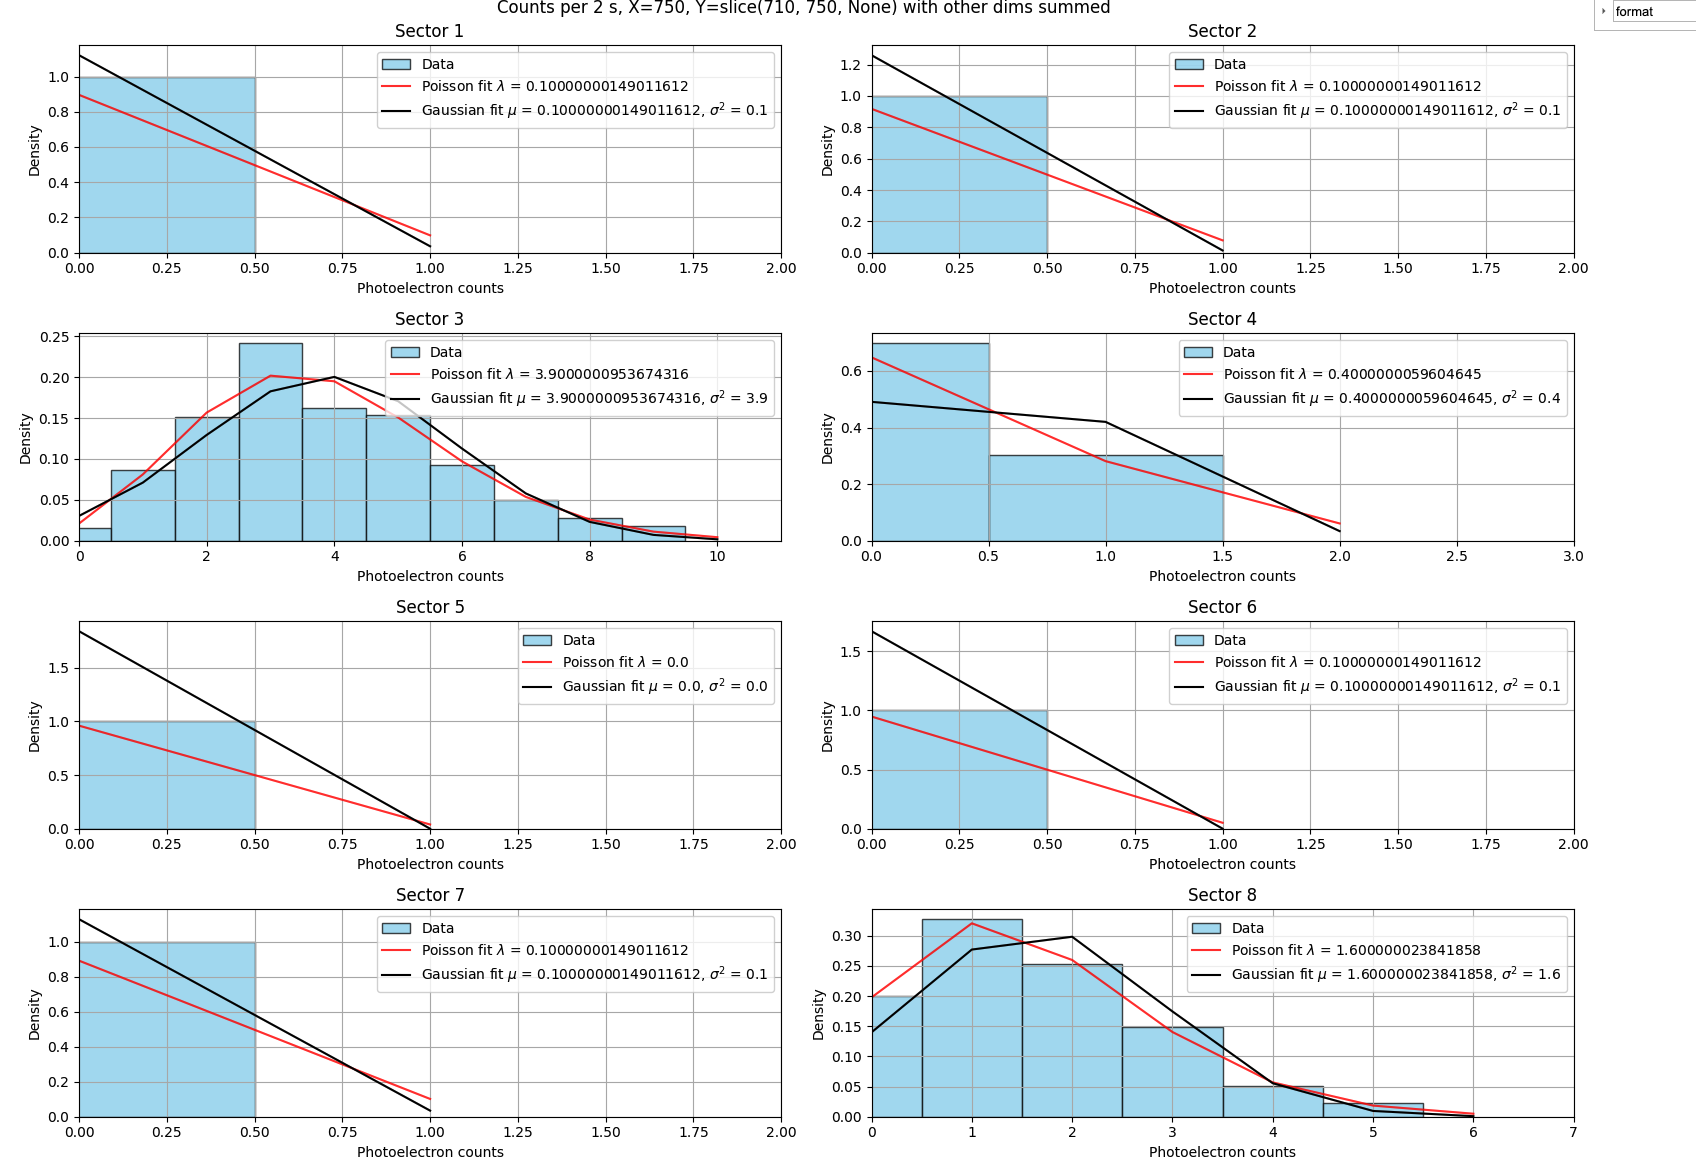
\includegraphics[width=1\linewidth]{images/poisson_stats/after_filtering_region_1000s.png}
    \caption{Data is filtered here with the KNN and looking at small region}
    % \label{fig:enter-label}
\end{figure}

\begin{figure}
    \centering
    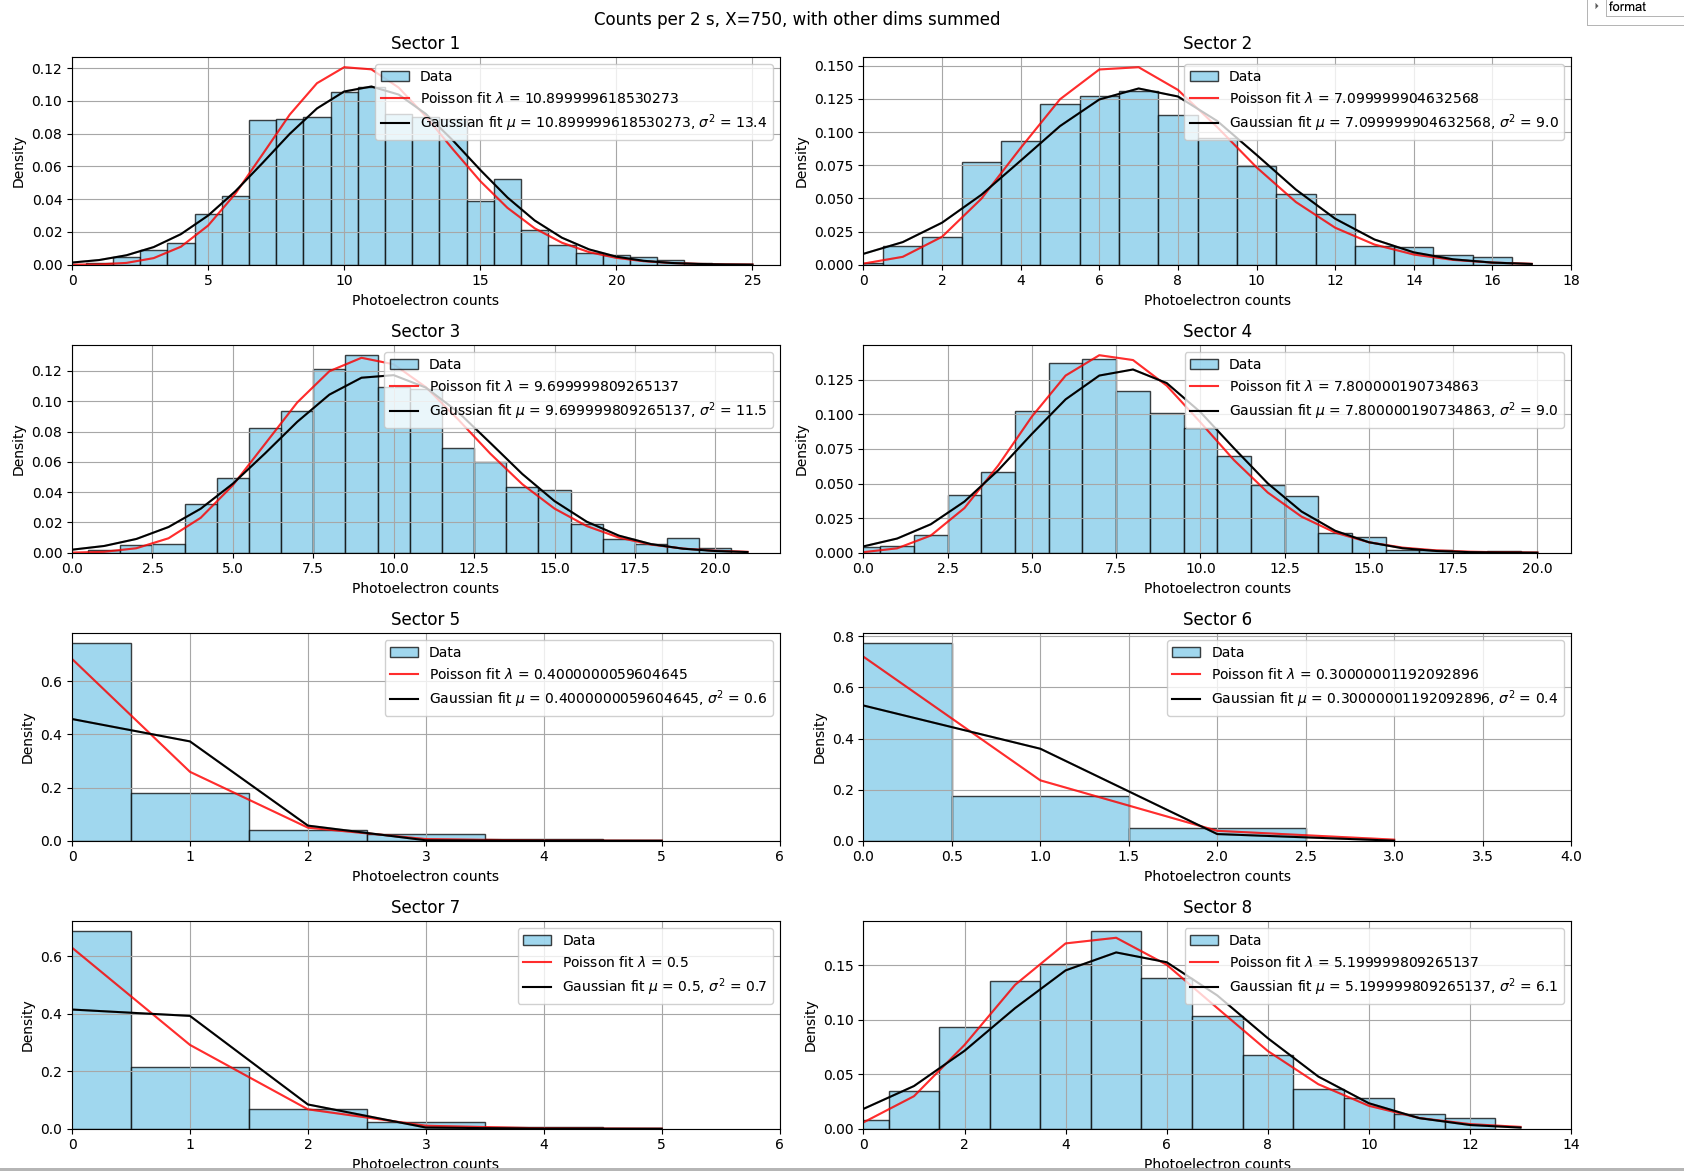
\includegraphics[width=1\linewidth]{images/poisson_stats/filtered_allY_singleX.png}
    \caption{Enter Caption}
    % \label{fig:enter-label}
\end{figure}


Taken from \cite{berteroImageDeblurringPoisson2009} which cites \cite{fellerIntroductionProbabilityTheory1968}
\section{Simulate Noise}
We simulate the data with Poissonian data.
\section{Statistical testing}

\begin{figure}[t]
    \centering
    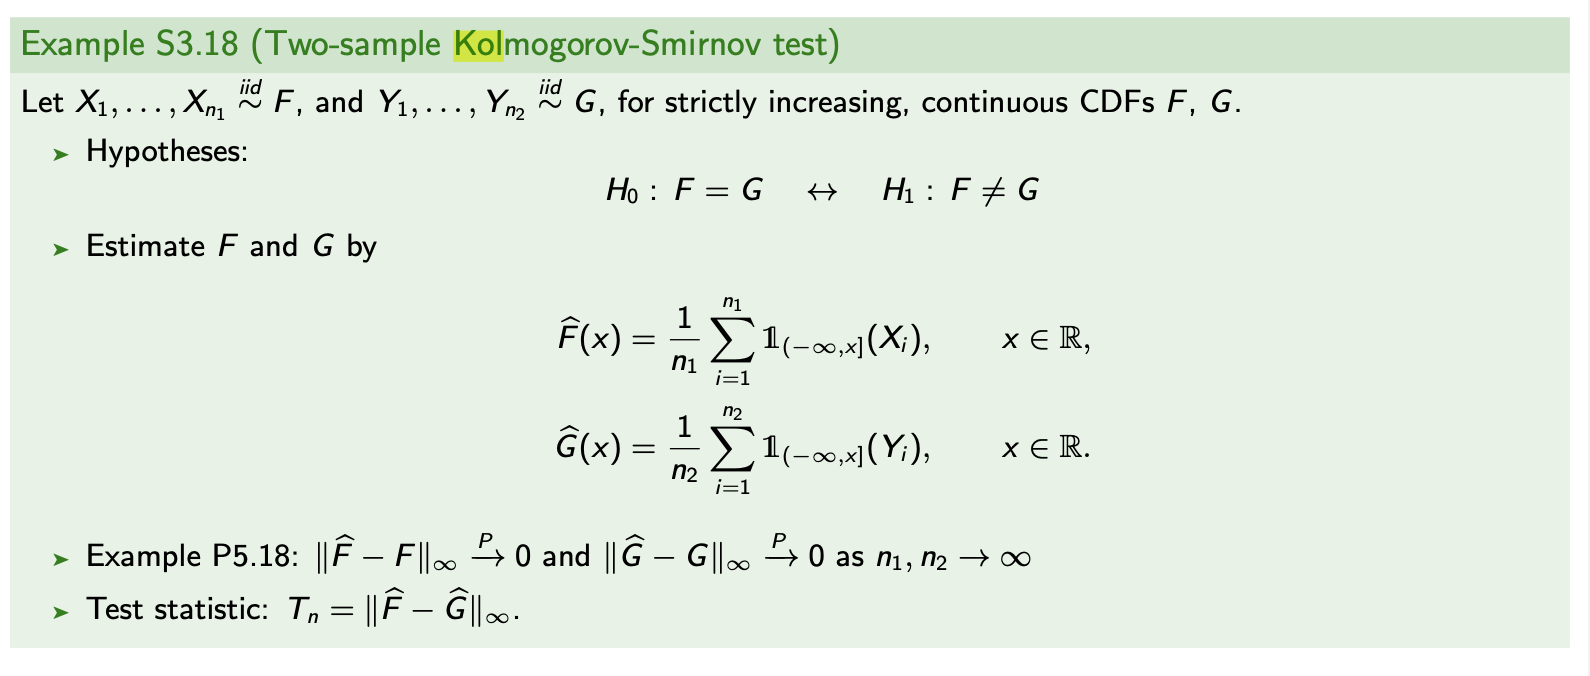
\includegraphics[width=1\linewidth]{images/2024-08-27-15.11.15.png}
    \caption{Enter Caption}
\end{figure}




\begin{figure}
    \centering
    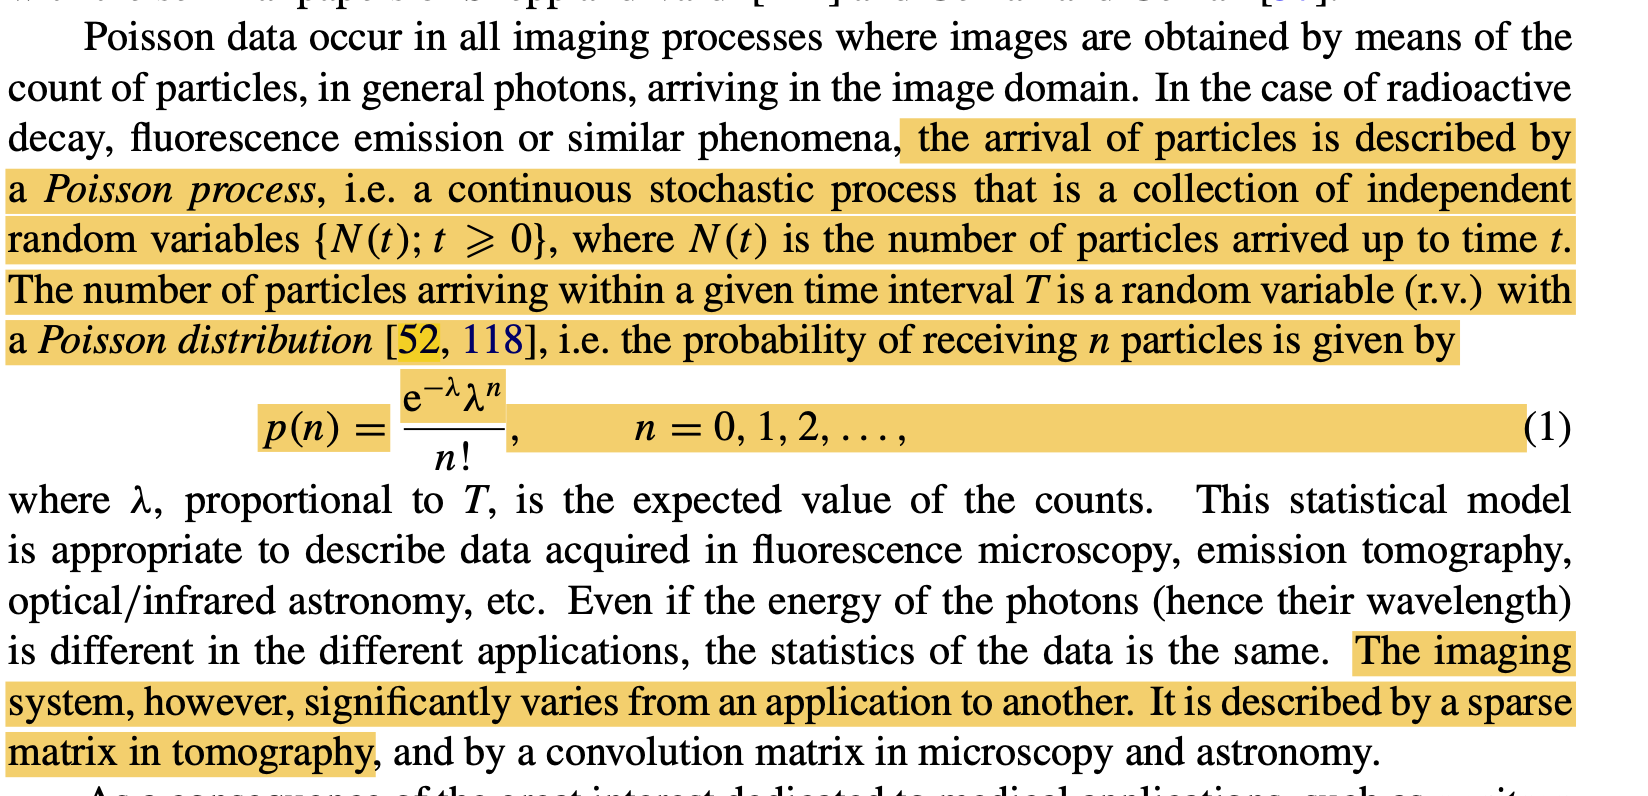
\includegraphics[width=1\linewidth]{images/JD-54-image.png}
    \caption{Enter Caption}
    \label{fig:enterl}
\end{figure}

% \section{Using CLT}
% Central Limit Theorem (CLT)
The \textbf{Central Limit Theorem} states that for a sequence of i.i.d. random variables \(X_1, X_2, \ldots, X_n\) with mean \( \mu \) and variance \( \sigma^2 \), the normalized sum of these variables approaches a standard normal distribution as \(n\) tends to infinity:

\[
\frac{\sum_{i=1}^{n} X_i - n\mu}{\sigma \sqrt{n}} \xrightarrow{d} N(0, 1) \quad \text{as} \quad n \to \infty.
\]

This convergence is in distribution.
\begin{quotation}
    From the law of large numbers, one can show that the relative fluctuations reduce as the reciprocal square root of the number of throws, a result valid for all statistical fluctuations, including shot noise. From Wikipedia
    
    Shot noise exists because phenomena such as light and electric current consist of the movement of discrete (also called "quantized") 'packets'.
\end{quotation}

Can't correlate FEL intensity with electron counts per pulse as the GMD is before the monochromator. 

\begin{quotation}
    The physical assumptions which we want to express mathematically are that the \textbf{conditions of the experiment remain constant} in time*, and that non-overlapping time intervals are stochastically independent in the sense that information concerning the number of events in one interval reveals nothing about the other. The theory of probabilities in a continuum makes it possible to express these statements directly, but being restricted to discrete probabilities, we have to use an approximate finite model and pass to the limit.

    Imagine a unit time interval partitioned into n subintervals of length 1/n. A given collection of finitely many points in the interval may be regarded as the result of a chance process such that each subinterval has the same probability $P_{n}$ to contain one or more points of the collection. A subinterval is then either occupied or empty, and the assumed independence of non-overlapping time intervals implies that we are dealing with Bernoulli trials: We assume that the probability for exactly k occupied subintervals is given by $b(k;n,P_{n})$. We now refine this discrete model indefinitely by letting n→inf. The probability that the whole interval contains no point of the collection must tend to a finite limit. But this is the event that no cell is occupied, and its probability is $(1-p_{n})^{n}$. Passing to logarithms it is seen that this quantity approaches a limit only if $np_{n}$
    from book \cite{fellerIntroductionProbabilityTheory1968}
\end{quotation}

\section{Chi-squared Goodness of Fit Test}
We hypothesize that the data follows a certain distribution e.g. Poisson, Normal, Negative Binomial The Chi-squared Goodness of Fit Test is used to determine if the observed data is consistent with the expected distribution.

Let \( X_1, X_2, \ldots, X_n \sim \text{i.i.d. } F \) and \( Y_1, Y_2, \ldots, Y_m \sim \text{i.i.d. } G \), where \( F \) and \( G \) are strictly increasing continuous \glsplural{CDF}.

The hypotheses for the chi-square test are:

\begin{equation}
    H_0: F = G \leftrightarrow   H_1: F \neq G
\end{equation}
The hypothesis test for the Poisson distribution is the Chi-squared Goodness of Fit Test. The test statistic is given by:

\begin{equation}
    \chi^2 = \sum_{i=1}^{k} \frac{(O_i - E_i)^2}{E_i}
\end{equation}
where \(O_i\) is the observed frequency and \(E_i\) is the expected frequency. The degrees of freedom are given by \(k-1\), where \(k\) is the number of bins.

For goodness-of-fit tests, small p-values indicate that you can reject the null hypothesis and conclude that your data were not drawn from a population with the specified distribution. Consequently, goodness-of-fit tests are a rare case where you look for high p-values to identify candidate distributions. 
(From \href{https://statisticsbyjim.com/hypothesis-testing/goodness-fit-tests-discrete-distributions/}{This website})


\begin{figure}[t]
    \centering
    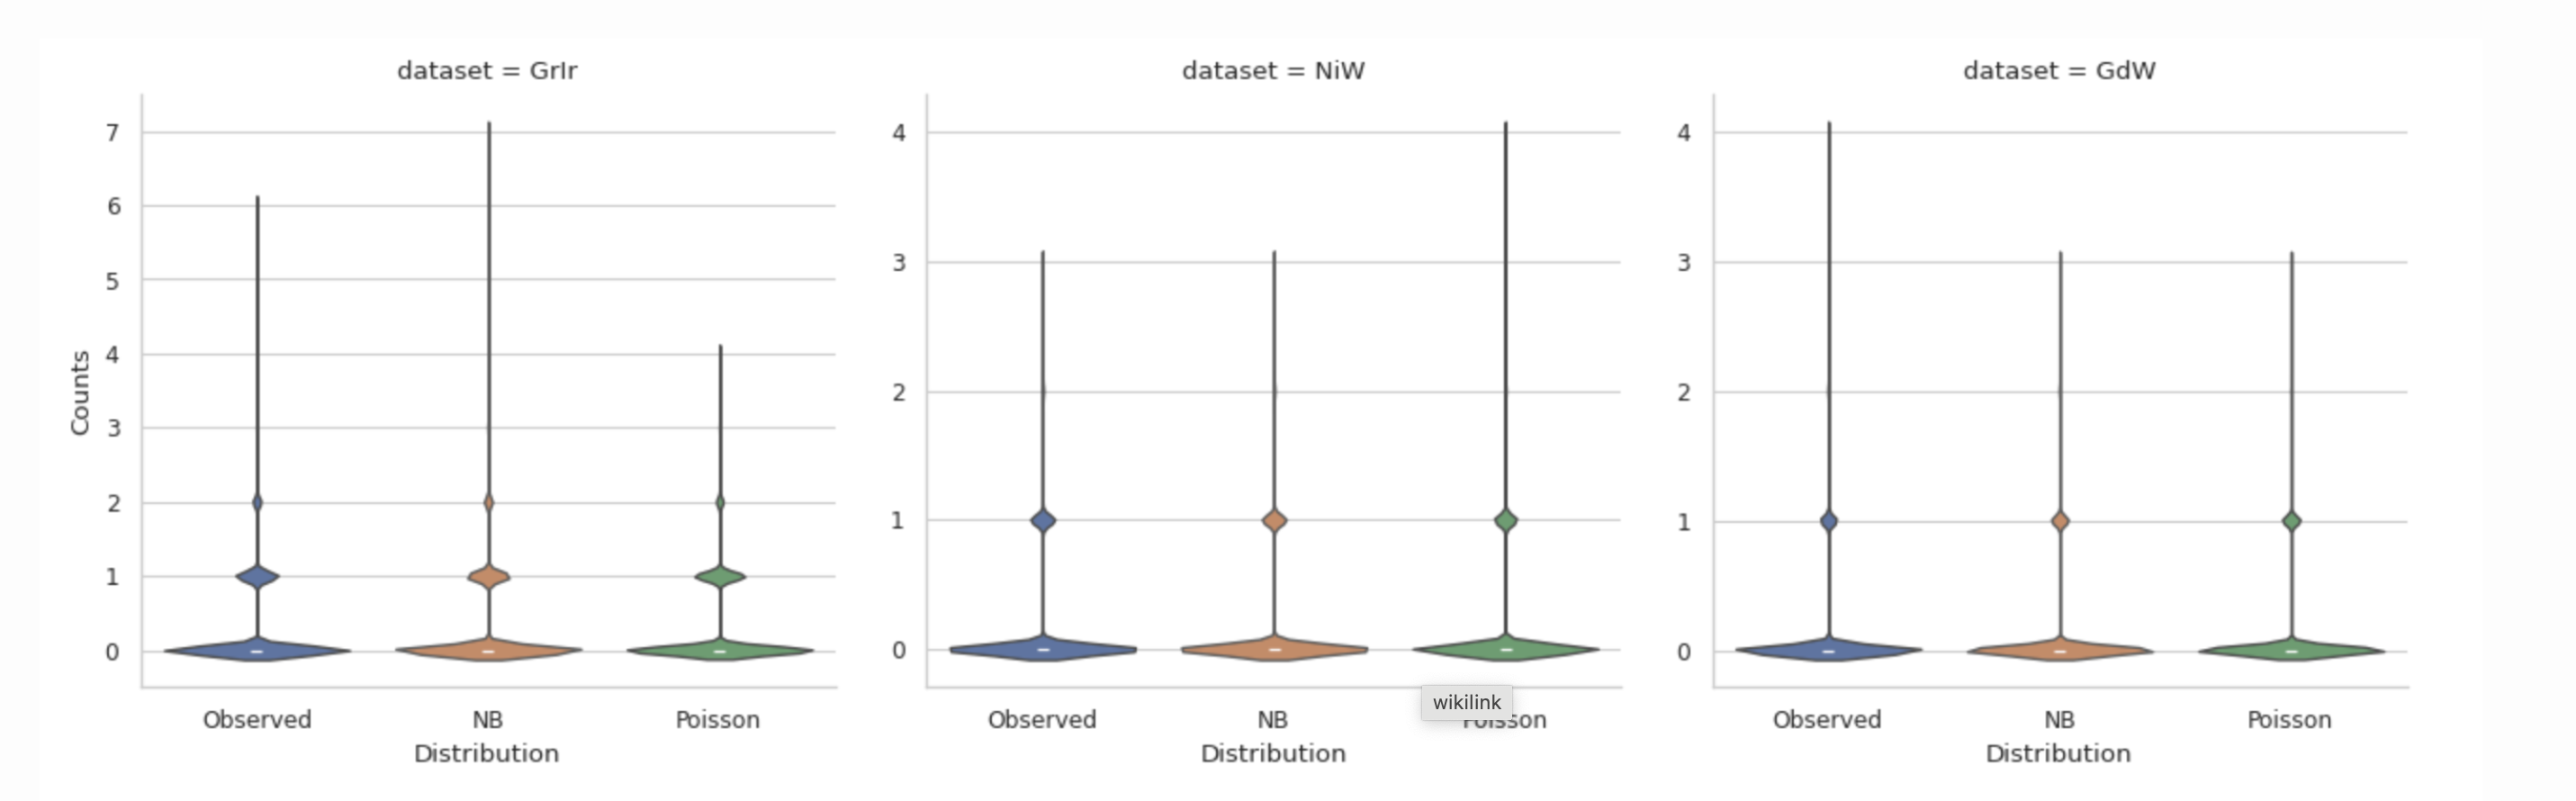
\includegraphics[width=1\linewidth]{images/violin_plots_per_pulse.png}
    \caption{Enter Caption}
\end{figure}

\begin{figure}[htbp]
    \centering
    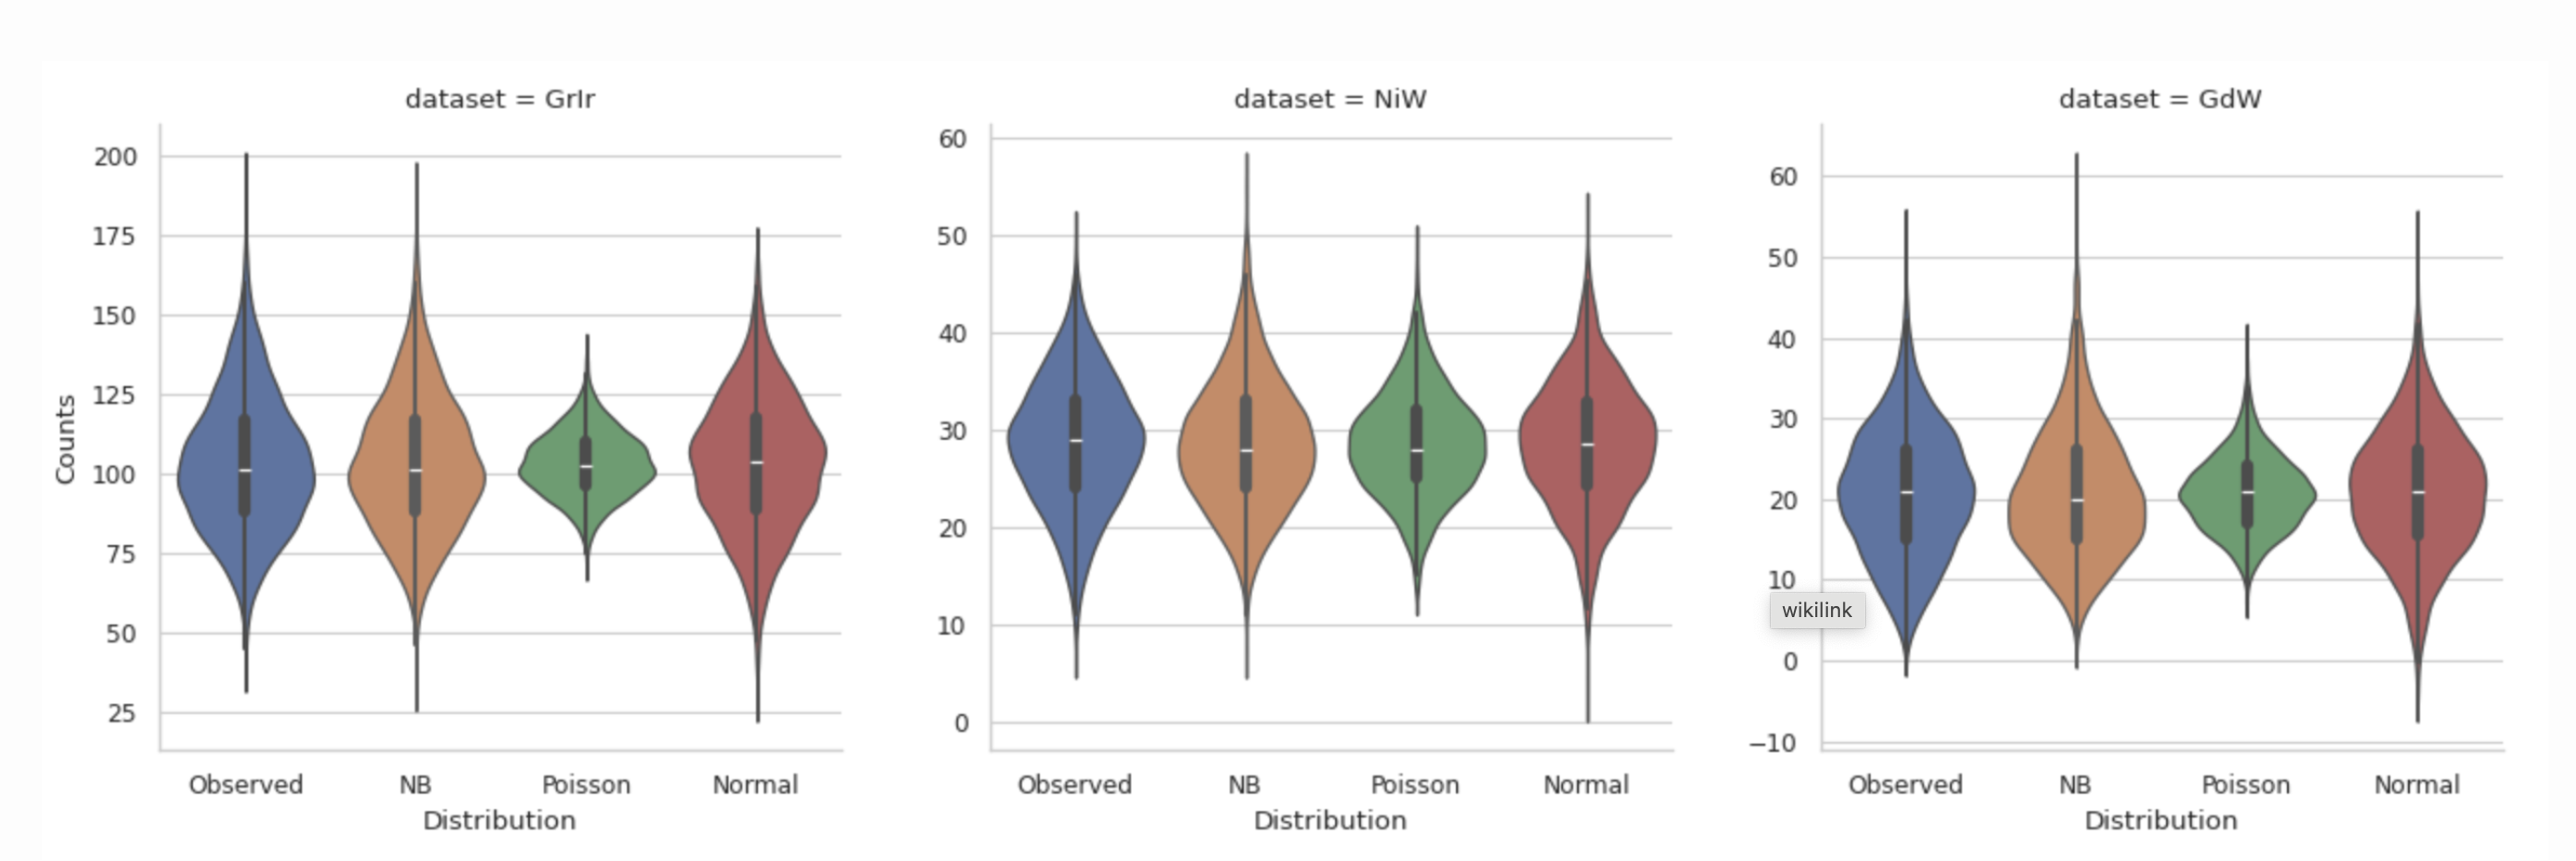
\includegraphics[width=1\linewidth]{images/violinplots_per_train.png}
    \caption{ss}
    \label{s}   
\end{figure}
\section{Modeling over-dispersed count data}

\section{The SASE process as an explanation of over-dispersed statistics}

